%%%%%%%%%%%%%%%%%%%%%%%%%%%%%%%%%%%%%%%%%%%%%%%%%%%%%%%%%%%%%%%%%%%%%%%%%%%%%%%
%% 3.- Pruebas y Resultados
%%%%%%%%%%%%%%%%%%%%%%%%%%%%%%%%%%%%%%%%%%%%%%%%%%%%%%%%%%%%%%%%%%%%%%%%%%%%%%%

\cleardoublepage
\chapter{Pruebas y Resultados}
\chaptermark{Pruebas y Resultados}

\label{chap:resultados} % etiqueta para poder referenciar luego en el texto con ~\ref{sec:intro}
% \addcontentsline{toc}{chapter}{Introducción, Objetivos, Metodología y Planificación}


\section{Pruebas control UTA}
\label{sec:pruebasUTA}

Tras realizar el programa y el diseño de la pantalla para el control de la UTA, estos se cargan en un simulador como el de la figura xxx, que se compone de un iPro y una pantalla para pruebas. Dado que el programa se ha simulado previamente en el software ISaGRAF, no se han encontrado problemas de funcionamiento en él, sin embargo, es habitual y así ha sido en este caso, encontrar errores de diseño en la pantalla, que se han pasado por alto durante su creación. Estos problemas se han corregido desde el software Visoprog y se han vuelto a cargar.

Cuando el resultado de las pruebas es bueno, desde fábrica realizan un cuadro nuevo con iPro, al que se le carga el programa realizado tras comprobar que el iPro funciona correctamente. Este cuadro se envía al cliente, en este caso el instalador al cargo del supermercado.


\section{Pruebas kiwi}
\label{sec:pruebasKiwi}

En las primeras pruebas del kiwi, se han descubierto varios problema y/o necesidades:

\begin{itemize}
  \item La necesidad de borrar la configuración guardada sin necesidad de acceder al portal web de configuración. Para ello se han añadido al programa las líneas necesarias para detectar la pulsación del botón integrado en la placa durante 5 segundos, lo que indica que se quiere resetear el kiwi y borrar la configuración realizada.
  \item En esa primera versión, no se disponía de la posibilidad de conexión por cable, pero se decidió añadir dicha opción dado que dependiendo del equipo y la instalación puede ser más rentable usar un dispositivo como el kiwi conectado vía ethernet.
  \item Timeout de mensajes. Cada vez que se recibían mensajes para un dispositivo, kiwi abría un canal para los mensajes destinados a ese dispositivo, pero no volvía a cerrarlo, por lo que se ha añadido un tiempo (timeout) tras el cual, si no se vuelven a recibir mensajes a través de ese canal, se vuelve a cerrar. 
  \item Problema de cambio de modo (AP y cliente). Para la gestión de la conexión de red, WiFi o Ethernet, se han empleado las librerías estándar para el ESP32: WiFi.h, ETH.h, WiFiClient.h. Al parecer estas librerías no gestionan bien el paso de un modo a otro, por lo que el ESP32 parecía dejar de funcionar. La solución ha sido reiniciar el kiwi tras la configuración, para volver a ponerse en marcha desde cero, en el nuevo modo, a partir de los parámetros de configuración guardados en la EEPROM.
  \item Desconexiones puntuales de la red WiFi. En el kiwi instalado para pruebas en la red de la empresa Intarcon, se detectaron desconexiones contínuas de la red WiFi. Este problema dio muchos dolores de cabeza, ya que el kiwi parecía funcionar sin problemas en otras redes. Para analizar este caso, se conectó un segundo kiwi en una red aislada, empleando un router de los empleados por kiconex para aquellas instalaciones sin acceso a la red, y se registraron en una hoja las desconexiones de ambos kiwis. \\ El resultado fue el de la \hyperref[figura:erroresIntarcon]{Figura~\ref{figura:erroresIntarcon}} y la \hyperref[figura:erroresRouter]{Figura~\ref{figura:erroresRouter}}, donde se puede ver que el kiwi de la red del router no tuvo ningún problema, mientras que el kiwi de la red de Intarcon tenía desconexiones contínuas durante el horario de trabajo: de 8 a 18:30. Fue este último dato el decisivo para saber que el problema estaba en la red de Intarcon, por lo que lo consultamos con el informático al cargo de la misma: nos confirmó que tras unos cambios en la red, había problemas con las DNS, y muchos equipos eran expulsados de la red. Este problema aun persiste, aunque en menor medida, pero el kiwi conectado al router sirve de muestra del buen funcionamiento del mismo.
\end{itemize}

\clearpage
\vspace*{\fill}
\begin{figure}[H]
  \centering
  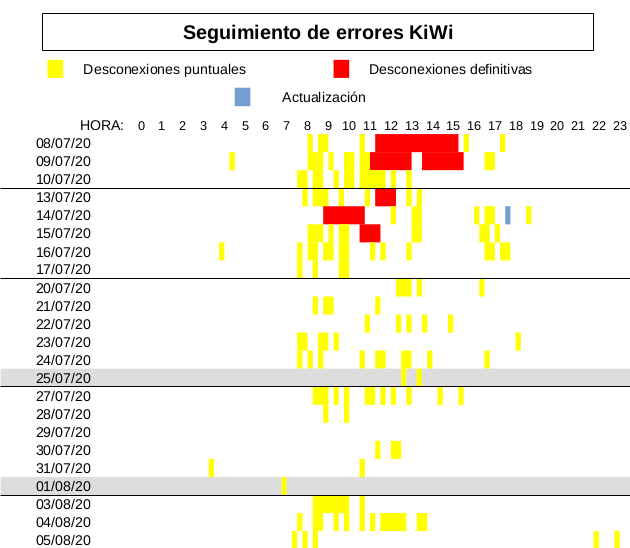
\includegraphics[width=\textwidth, keepaspectratio]{img/erroresRedIntarcon}
  \caption{Desconexiones kiwi en red de Intarcon}
  \label{figura:erroresIntarcon}
\end{figure}
\vspace*{\fill}

\clearpage
\vspace*{\fill}
\begin{figure}[H]
  \centering
  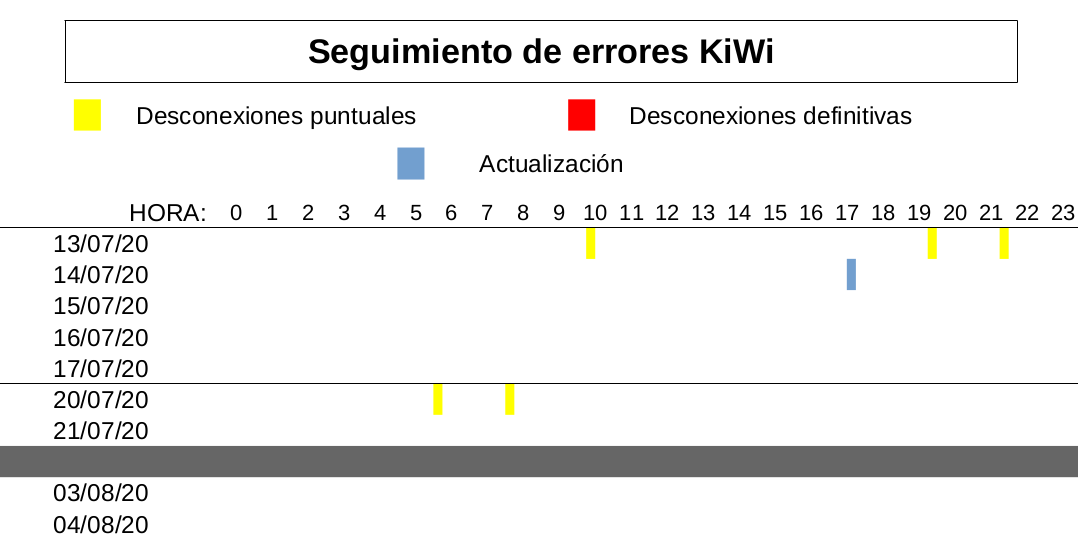
\includegraphics[width=\textwidth, keepaspectratio]{img/erroresRedRouter}
  \caption{Desconexiones kiwi en red de router kiconex}
  \label{figura:erroresRouter}
\end{figure}
\vspace*{\fill}
\clearpage

\section{Puesta en marcha de la instalación}
\label{sec:altaInstalación}

Cuando se conectan todos los dispositivos de la instalación, es momento de su puesta en marcha y de comprobar que todo está correctamente. Se trata de un trámite necesario, ya que aunque normalmente no da problemas, existen ocasiones en las que falla la conexión por causas ajenas a kiconex: resistencias de extremo de cable modbus, direcciones Modbus no configuradas en los equipos correctamente, etc. En este caso, el mapa de direcciones Modbus es el de la \hyperref[tab:direccionesModbus]{Tabla~\ref{tab:direccionesModbus}}.

\vspace*{\fill}

\begin{table}[H]
  %\centering
  \begin{center}
    \setlength\arrayrulewidth{2pt}
    \begin{tabular}{| r | c |}
      \hhline{|*{2}{-}}
      \cellcolor{lightgray}\textbf{\footnotesize{EQUIPO}} & \cellcolor{lightgray}\textbf{\footnotesize{DIRECCIÓN}}\\ \hline
      \footnotesize{Cámara BT} & 1 \\ \hline
      \footnotesize{Cámara MT} & 2 \\ \hline
      \footnotesize{Cámara AT} & 3 \\ \hline
      \footnotesize{Isla BT} & 4 \\ \hline
      \footnotesize{Vitrina MT} & 5 \\ \hline
      \footnotesize{Murales MT} & 6 \\ \hline
      \footnotesize{Semimurales MT} & 7 \\ \hline
      \footnotesize{Obrador MT} & 8 \\ \hline
      \footnotesize{Unidad de Tratamiento de Aire} & 9 \\ \hline
      \footnotesize{Central de Refrigeración} & 10 \\ \hline
      \footnotesize{Bomba de calor} & 11 \\ \hline
    \end{tabular}
    \caption{Direcciones Modbus equipos supermercado.}
    \label{tab:direccionesModbus}
  \end{center}
\end{table} 

\vspace*{\fill}

La \hyperref[figura:instalcionConectada]{Figura~\ref{figura:instalcionConectada}} muestra como todos los elementos de la instalación se han conectado correctamente.

\clearpage
\vspace*{\fill}

\begin{figure}[H]
  \centering
  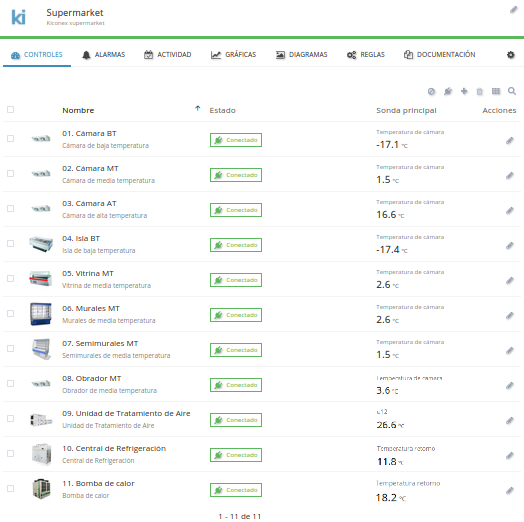
\includegraphics[width=\textwidth, keepaspectratio]{img/instalacionConectada}
  \caption{Instalación supermercado conectada y funcionando}
  \label{figura:instalcionConectada}
\end{figure}

\vspace*{\fill}